% ==============================================================================
% TCC - Nome do Aluno
% Capítulo 2 - Referencial Teórico
% ==============================================================================
\chapter{Referencial Teórico}
\label{sec-referencial}

No decorrer deste capítulo serão apresentados conceitos usados como base para o desenvolvimento deste trabalho: um breve resumo sobre Engenharia de Requisitos (Seção~\ref{sec-ref-engenharia-requisitos}), uma descrição sobre a Engenharia \textit{Web}, alguns de seus atributos técnicos de qualidade e as fases seguidas por uma abordagem iterativa (Seção~\ref{sec-ref-engenharia-web}); o método FrameWeb, suas propostas, suas divisões através de camadas e a utilização de uma linguagem específica de modelagem (Seção~\ref{sec-ref-frameweb}). O capítulo também aborda uma visão sobre as categorias dos \textit{frameworks}, uma descrição sobre o \textit{framework} Grails utilizado no projeto e a linguagem Groovy que é utilizada por ele (Seção~\ref{sec-ref-frameworks}).


\section{Engenharia de Requisitos}
\label{sec-ref-engenharia-requisitos}

Considerados um fator determinante para o fracasso ou sucesso de um projeto de \textit{software}, os requisitos desempenham um papel central no processo de \textit{software}. De modo geral, é possível dizer que os requisitos de um sistema incluem restrições sob as quais ele deve operar, restrições que devem ser satisfeitas no seu processo de desenvolvimento, especificações dos serviços que o sistema deve prover e propriedades gerais do sistema~\cite{falbo:er17}.

Os requisitos podem ser definidos como as descrições das restrições operacionais e dos serviços que devem ser providos pelo sistema~\cite{sommerville:es07}. Com relação ao tipo de informação documentada por um requisito, uma classificação é amplamente aceita e de acordo com~\citeonline{sommerville:es07}, os \textbf{requisitos funcionais} são declarações de serviços que o sistema deve prover, descrevendo o que o sistema deve fazer. Já os \textbf{requisitos não funcionais}, descrevem restrições sobre os serviços ou funções oferecidas pelo sistema. Neste contexto, ainda existem as regras de negócio, que definem requerimentos e restrições do negócio, sendo particulares para cada cliente.

Uma tarefa bem útil é representar os requisitos em níveis diferentes de descrição, pois os desenvolvedores, os clientes que contratam o desenvolvimento do sistema e os usuários finais são muito interessados em requisitos, mas possuem expectativas distintas. Assim,~\citeonline{sommerville:es07} realiza a descrição de dois níveis de requisitos:

\begin{itemize}
	\item \textbf{Requisitos de Usuário ou de Cliente:} devem ser de fácil entendimento para clientes e usuários do sistema que não possuem conhecimento técnico. São diagramas intuitivos das restrições e dos serviços esperados do sistema, todos através da utilização de linguagem natural.
	
	\item \textbf{Requisitos de Sistema:} especificam em detalhes as restrições, serviços e funções do sistema, produzindo uma versão melhorada dos requisitos de clientes que os desenvolvedores utilizam para implementar, projetar e testar o sistema. 
\end{itemize}

Em seguida, as funcionalidades que um sistema deve prover podem ser capturadas e descritas pelos modelos de casos de uso. Na maioria das vezes, um sistema atende a vários atores e por este motivo, analisar a funcionalidade que ele provê como uma única unidade pode ser uma tarefa complicada. O conceito de caso de uso tem a utilidade de dividir essa funcionalidade em partes mais agradáveis e menores~\cite{olive:cmis07}.

Então, com a responsabilidade de relacionar as necessidades e as exigências do cliente, a fase de análise de requisitos se segue e estabelece atividades para que seus objetivos sejam atingidos através de soluções que deverão ser implementadas e entregues em um produto final de \textit{software}. Desta maneira, a análise de requisitos engloba a compreensão dos estudos das necessidades e das solicitações do usuário para que as soluções sejam desenvolvidas. Resumidamente, a análise de requisitos envolve o entendimento do problema, sua avaliação, uma estratégia para a solução, sua modelagem, a especificação dos requisitos e a devida validação~\cite{amui:pds15}.

Diferentes objetos desempenham um mesmo papel no mundo real, compartilhando um mesmo comportamento e uma mesma estrutura. Não existe a necessidade de realizar a modelagem de cada objeto individualmente, pois é mais vantajoso reunir em apenas um lugar, um modelo que descreve o comportamento e a estrutura desses objetos. Esse modelo passa a se tornar uma classe. Uma classe descreve um conjunto de objetos com os mesmos atributos, associações, operações e a mesma semântica. Portanto, a modelagem orientada a objetos é constituída pela definição de classes~\cite{falbo:er17}.

Além de organizar as classes em um diagrama, esta fase também identifica restrições de integridade, que são limitações às possíveis soluções no desenvolvimento referente ao produto a ser entregue e não ao projeto em si. Elas não representam os requisitos de forma direta, mas induzem à definição de requisitos específicos. As restrições afetam a construção, o desenho da solução, a validação, os testes e a implantação do \textit{software}, não podendo sofrer alterações. Por este motivo, elas devem ser muito bem validadas~\cite{vazquez-et-al:erson16}.

Após especificados os requisitos, se seguem atividades de projeto e implementação de \textit{softwares}, que são invariavelmente intercaladas. O projeto de \textit{software} é uma atividade criativa aonde são identificados os componentes de \textit{software} e seus relacionamentos de acordo com os requisitos do cliente. A implementação estabelece o processo de concretização do projeto como um programa. Sempre existe um processo de projeto, pois um projeto trata de como resolver um problema. O projeto e a implementação estão intimamente ligados e, ao elaborar um projeto, é necessário levar em consideração os problemas de implementação que serão enfrentados~\cite{sommerville:es11}.



\section{Engenharia \textit{Web}}
\label{sec-ref-engenharia-web}

A \textit{Web} é uma ferramenta que dispensa apresentações, pois ela já está familiarizada entre a maioria das pessoas, se encontra presente no dia a dia e em quase todas as áreas, podendo ser acessada através de muitos \textit{hardwares} diferentes. Inicialmente, o conteúdo de \textit{websites} era apenas textual, estático e não existia a presença de animações, sons, imagens ou conteúdo gerado de maneira dinâmica para cada tipo de usuário. A preocupação dos desenvolvedores permanecia em torno da simplicidade de apenas visualizar as informações sem complexidades.

Com a evolução de forma acelerada da \textit{web}, surgiu a necessidade de mudanças significativas na maneira como os \textit{websites} eram criados. Os \textit{websites} passaram a englobar diversos conteúdos e funções complexas, adicionando centenas ou milhares de objetos em seu contexto. Sendo assim, quando toda a adição desses conteúdos começou a gerar um impacto direto no sucesso dos negócios, os projetos \textit{web} deixaram de ser tratados de maneira superficial~\cite{pressman:es11}.

Acompanhando as evoluções do mundo, diversos setores onde não se imaginava uma maneira de como a \textit{web} poderia ser utilizada, foram obrigados a adotar essa tecnologia para poderem se manter no mercado, se equiparando com a concorrência existente. Se antes era preciso concentrar e controlar todos os sistemas de forma interna e não unificada, atualmente já é possível realizar a terceirização de serviços, como por exemplo: o controle de banco de dados, o gerenciamento de e-mails, o controle de inúmeros \textit{hardwares} de maneira remota, entre outros.

Algumas aplicações passaram a desempenhar um papel muito importante nas organizações, como por exemplo: as aplicações de instituições financeiras, que não toleram nenhum tipo de erro em sua utilização. Assim, os problemas encontrados nas aplicações \textit{Desktop}, também passaram a ser visualizados nas aplicações para a \textit{web}. Alguns fatores como a falta de qualificação e a falta de experiência dos desenvolvedores, a não utilização de modelos de processo, a não utilização de métricas para estimativas, se somavam para encadear os problemas encontrados. Além disso, o planejamento incoerente, os métodos obsoletos e inadequados, o não cumprimento de custos e prazos, a falta de documentação e o não cumprimento dos requisitos, dificultavam muito o controle da qualidade das aplicações~\cite{peruch-pg07}.               

Neste contexto de atualizações globais, à medida que a complexidade dos \textit{websites} foi aumentando, eles passaram a ser considerados verdadeiras aplicações na \textit{web}, sendo necessário utilizar os fundamentos da Engenharia \textit{Web}, que pode ser definida como a utilização de conceitos, princípios e métodos da Engenharia de Software, de modo que estabeleçam uma maneira de realizar adaptações referentes às características das aplicações \textit{web}~\cite{beder:ew12}.

Existem atributos técnicos de qualidade que são utilizados na Engenharia de Software. A usabilidade visa a facilidade de utilização da aplicação, independente do tipo de usuário. A funcionalidade faz referência ao comportamento do sistema, buscando operações e informações corretamente. A eficiência é voltada para o tempo de resposta, retornando as informações em uma velocidade satisfatória. A confiabilidade deve garantir a recuperação de erros e validação das informações e a manutenibilidade deve garantir a fácil atualização das operações existentes na aplicação. Todos esses atributos podem ser utilizados no desenvolvimento de aplicações \textit{web}. De acordo com \citeonline{offutt:eis02}, os principais atributos técnicos de qualidade podem ser extendidos através de outros atributos: 

\begin{itemize}
	
	\item \textbf{Segurança:} existem inúmeras informações confidenciais que são armazenadas e extraídas através das \textit{WebApps}, além de existir a integração com bancos de dados governamentais e corporativos. Por estes motivos, assim como outros, em inúmeras situações, a segurança da \textit{WebApp} deve ser tratada com prioridade. Para estabelecer o atributo de segurança, a \textit{WebApp} deve possuir a habilidade de se defender contra ataques maldosos e bloquear solicitações que não possuem acesso autorizado;
	
	\item \textbf{Disponibilidade:} uma \textit{WebApp} indisponível não tem serventia nenhuma para os usuários, mesmo que ela seja de extrema qualidade. A disponibilidade é definida pelo percentual de tempo que a aplicação fica disponível para uso. Os usuários sempre esperam que as \textit{WebApps} fiquem disponíveis a todo o momento, no entanto, a disponibilidade também está relacionada com os tipos de plataformas diferentes que as \textit{WebApps} são compatíveis;

	\item \textbf{Escalabilidade:} os servidores e as \textit{WebApps} não podem ser projetados para um número fixo de usuários. A capacidade de volume e a capacidade de resposta devem ser levadas em consideração durante a construção, ou seja, variações significativas podem ocorrer a qualquer momento. Um número bem grande de usuários devem ser esperados no futuro;

	\item \textbf{Tempo de inserção no mercado:} do ponto de vista comercial, é uma boa medida de qualidade. Geralmente, um número variável de usuários são atraídos pelas primeiras \textit{WebApps} que atendem um segmento específico de mercado. O usuário fica responsável por realizar a avaliação da qualidade da \textit{WebApp};

\end{itemize}

O desenvolvimento de uma \textit{WebApp} é uma atividade com características variadas, envolvendo questões organizacionais, técnicas, gerenciais, artísticas e sociais. Reunindo um conjunto de atividades aplicadas, o objetivo é gerar uma aplicação de qualidade que atenda as características esperadas de forma eficiente.

Ao iniciar um projeto de uma \textit{WebApp}, a Engenharia \textit{Web} estabelece algumas fases para que uma abordagem iterativa seja seguida. Essas fases são aplicadas de acordo com que o projeto se desenvolve. Se repetindo quantas vezes forem as iterações do projeto, as fases de comunicação, planejamento, modelagem, construção e emprego, produzem um incremento de \textit{software} a cada iteração, disponibilizando uma parte das funcionalidade e dos recursos do \textit{software}, se tornando bem mais completo~\cite{pressman:es11}.

\subsection{Comunicação}
\label{sec-ref-comunicacao}

De início temos a fase de \textbf{comunicação}, onde é necessário compreender os objetivos das partes interessadas, conhecendo as restrições e necessidades do \textit{software}, documentando o registro da análise e realizando a verificação, validação e gerenciamento dos requisitos. Além disso, os requisitos de qualidade, interface de usuário, ambiente de sistema e conteúdo também devem ser tratados, assim como requisitos não-funcionais.

\subsection{Planejamento}
\label{sec-ref-planejamento}

Em sequência, é descrita a fase de \textbf{planejamento}, em que as tarefas técnicas a serem conduzidas devem ser descritas, assim como os recursos que serão utilizados, um cronograma de trabalho, os riscos prováveis e os resultados esperados dos produtos. Através dos requisitos especificados, os elementos da arquitetura são definidos através de uma transmissão entre a análise de contexto e o desenvolvimento do sistema.

\subsection{Modelagem}
\label{sec-ref-modelagem}

Na fase de \textbf{modelagem}, os padrões e as normas são definidas para realizar a organização do desenvolvimento do sistema, acrescentando detalhes para que o problema e a solução proposta sejam compreendidos da melhor maneira possível. As transições entre as fases e os métodos de realização também são definidos, abordando todas as questões globais do projeto.   

\subsection{Construção}
\label{sec-ref-construcao}

Posteriormente, na fase de \textbf{construção}, é preciso transformar toda a lógica, operações e o controle do sistema em código-fonte, utilizando uma linguagem de programação determinada. O conteúdo da aplicação, o aspecto visual e os elementos de navegação são definidos e testes são realizados para revelar possíveis erros na implementação do código. 

\subsection{Emprego}
\label{sec-ref-emprego}

Por fim, na fase de \textbf{emprego}, a aplicação é entregue ao cliente, em partes que serão incrementadas ou completa, para que ele realize a avaliação do produto. A aplicação deve ser mantida sempre atualizada e permitir uma manutenibilidade fácil para garantir que esteja sempre disponível e seja funcional. Nesta fase ainda podem ocorrer mudanças estruturadas ou não estruturadas.

\section{O Método FrameWeb}
\label{sec-ref-frameweb}

Utilizando \textit{frameworks} como base, o FrameWeb (\textit{Framework-based Design Method for Web Engineering})~\cite{souza:masterthesis07,souza-celebratingfalbo20} é um método de projeto voltado para o desenvolvimento de sistemas de informação \textit{Web} (\textit{Web Information Systems} - WISs). Ao se desenvolver aplicações distribuídas, especialmente as baseadas na plataforma \textit{Web}, o uso de \textit{frameworks} se padronizou, passando a existir inúmeras propostas para a Engenharia \textit{Web}. Mesmo com muitos \textit{frameworks} existentes, assim como métodos e metodologias, não havia nada que englobasse diretamente as características dos \textit{frameworks} utilizados no desenvolvimento de WISs. O método FrameWeb surgiu com o intuito de propor modelos de projetos que chegam perto da implementação do sistema, definindo uma arquitetura básica para o WIS e assumindo que determinados tipos de \textit{frameworks} serão utilizados no decorrer da construção da aplicação.

Voltado para a fase de projeto arquitetural, o FrameWeb visa deixar as organizações e os desenvolvedores com a opção de adotar as técnicas mais adequadas para as demais etapas do processo. Nesta fase, as principais propostas do método são estabelecidas:
  
\begin{itemize}
	
	\item Divisão do sistema em camadas, através de uma arquitetura padrão, de modo a realizar uma integração com os \textit{frameworks} utilizados;
	
	\item Construção de modelos de projeto que reúnem conceitos utilizados pelos \textit{frameworks}, através de um perfil UML que traga os diagramas para mais perto da implementação.

\end{itemize}

O FrameWeb propõe o uso de uma arquitetura lógica do sistema, que seja estabelecida pelo padrão arquitetônico \textit{Service Layer} (Camada de Serviço)~\cite{fowler:peaa02}, representado na Figura~\ref{fig-ref-service-layer}. O sistema é dividido em três camadas grandes que são subdivididas internamente por pacotes:                            

\begin{figure}[h]
	\centering
	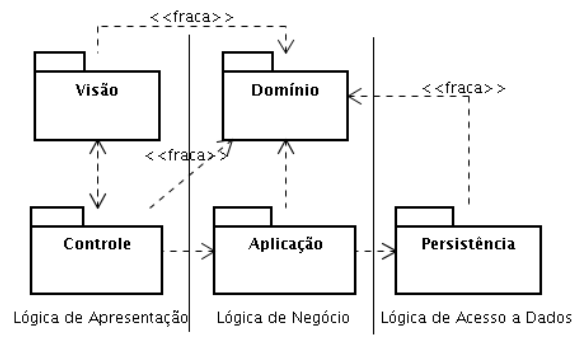
\includegraphics[scale=.6]{figuras/fig-ref-service-layer} 
	\caption{Arquitetura padrão para WIS baseada no padrão arquitetônico \textit{Service Layer}~\cite{fowler:peaa02}.}
	\label{fig-ref-service-layer}
\end{figure}

\begin{itemize}

	\item \textbf{Lógica de Apresentação:} possui a responsabilidade de realizar a interação entre o sistema e o usuário, exibindo as informações e interpretando os comandos em ações da persistência de dados e da lógica de negócio.
		
		\subitem -- Pacote de \textbf{Visão:} realiza a iteração humano-computador, definindo o formato de relatórios, formulários e janelas, sendo que a construção de protótipos é muito útil para facilitar o desenvolvimento dos mecanismos que serão utilizados. 
		
		\subitem -- Pacote de \textbf{Controle:} define as classes que serão responsáveis por controlar a iteração, enviando requisições para os objetos da Lógica de Negócio.  
	
	\item \textbf{Lógica de Negócio:} engloba as funcionalidades que dão suporte aos processos de negócio, concentrando as regras de negócio, conceitos do domínio, cálculos e processamentos.
	
		\subitem -- Pacote de \textbf{Domínio:} reúne o relacionamento direto entre os diagramas de classes produzidos na fase de análise e os conceitos do domínio do problema. 
		
		\subitem -- Pacote de \textbf{Aplicação:} está ligado ao modelo de casos de uso e é projetado de maneira independente da interface com o usuário.
	
	\item \textbf{Lógica de Acesso a Dados:} estabelece o acesso a dados, gerenciando requisições e cuidando da sincronização de elementos de dados.
	
		\subitem -- Pacote de \textbf{Persistência:} contém as classes que são responsáveis por gravar os objetos de domínio que necessitam ser persistidos pelo sistema em um banco de dados. O método FrameWeb sugere que as classes sigam o padrão de projeto \textit{Data Access Object} (DAO)~\cite{alur-et-al:bpds03}. Este padrão determina uma interface de operações de persistência, incluindo métodos para a criação, recuperação, alteração e exclusão, agrupando o código relacionado à entidade persistente~\cite{bauer-et-al:jpwh07}. 

\end{itemize}

%\subsection{Linguagem de Modelagem}
%\label{sec-ref-linguagem-modelagem}

Com o objetivo de representar de maneira direta os conceitos existentes nos \textit{frameworks} que podem ser integrados, o uso de uma linguagem específica de modelagem se tornou necessária~\cite{martins-souza:webmedia15}, pois os artefatos que serão codificados pelos desenvolvedores após a fase de projeto também devem ser modelados. O FrameWeb apresenta uma linguagem de modelagem que estende o meta-modelo UML, representando os componentes relacionados aos \textit{frameworks} e os componentes mais utilizados no desenvolvimento \textit{Web}. Um perfil UML é utilizado para a construção de quatro tipos de diagramas: 

\begin{itemize}  

	\item \textbf{Modelo de Entidades:} partindo do modelo de classes desenvolvido na fase de análise, os objetos de domínio do problema que serão persistidos no banco de dados são representados por um diagrama de classes da UML. Além disso, os mapeamentos que guiam a persistência dos objetos destas classes são adicionados;
	
	\item \textbf{Modelo de Persistência:} um diagrama de classes da UML representa a implementação das classes DAO existentes no sistema e que serão persistidas, exibindo todas as implementações das interfaces, assim como os seus respectivos métodos;
	
	\item \textbf{Modelo de Navegação:} demonstra as páginas \textit{Web} do sistema, seus atributos e suas iterações, exibindo o funcionamento dos inúmeros componentes que formam a camada de Lógica de Apresentação. Além disso, ele estabelece a maneira como cada categoria de usuário irá navegar de um elemento da \textit{WebApp} para outro. A mecânica de navegação é definida como parte do projeto, sendo necessário observar a definição e se concentrar nos requisitos gerais de navegação~\cite{pressman:es11}.	
	
	\item \textbf{Modelo de Aplicação:} exibe através de um diagrama de classes da UML, as classes de serviço, que implementam os casos de uso e as suas dependências. Esse diagrama é utilizado para auxiliar os desenvolvedores na implementação das classes do pacote Aplicação e na configuração das dependências entre os pacotes Controle, Aplicação e Persistência. Assim, é possível definir quais DAOs são necessários para que as classes de serviço alcancem seus objetivos e quais classes de ação dependem de quais classes de serviço~\cite{souza:masterthesis07}.

De acordo com~\citeonline{souza:masterthesis07}, se existirem classes de ação que dependem de uma classe de serviço exibida, elas também devem estar presentes no modelo, realizando a representação através da indicação da dependência por meio de uma associação direcionada à interface da classe de serviço e de espaços de nomes que pertencem a outro pacote. Portanto, quando a classe de serviço depende de algum DAO, a interface deste deve aparecer no diagrama e estar associada à classe de serviço em questão.	

\end{itemize}

A definição da linguagem de modelagem permite, ainda, a criação de ferramentas de apoio ao método, como um editor gráfico~\cite{campos-souza:webmedia17} e um gerador de código~\cite{almeida-et-al:webmedia17}. O FrameWeb Editor estabelece um ambiente gráfico para a criação de modelos FrameWeb, apresentando suas funcionalidades e aspectos relevantes de sua implementação.  



\section{Frameworks}
\label{sec-ref-frameworks}

Para realizar a implementação de um WIS, através da Engenharia \textit{Web}, o que mais se pode encontrar são ferramentas, propostas de metodologias e inúmeras linguagens que facilitam o processo realizado pelos desenvolvedores. Após a construção dos primeiros sistemas, verificou-se que os WISs possuíam uma infraestrutura arquitetônica bem parecida. Desta maneira, diversos \textit{frameworks} foram criados para generalizar essa infraestrutura e para facilitar a realização do desenvolvimento de novas aplicações.

Assim, um \textit{framework} pode ser considerado um design reutilizável de uma parte ou de todo o sistema, sendo representado por um conjunto de classes abstratas e concretas que demonstram a forma como suas instâncias interagem com um grande potencial de especialização~\cite{mattsson-et-al:csef99}. Com a utilização das funcionalidades que os \textit{frameworks} oferecem, a implementação dos códigos fontes das aplicações se tornam bem mais simples, minimizando os custos e o tempo utilizado.

Diversos \textit{frameworks} foram criados para a plataforma Java e após a construção de inúmeros WISs, \citeonline{souza:masterthesis07} estabeleceu uma organização para os \textit{frameworks} em seis categorias diferentes:    

\begin{itemize} 
	
	\item \textit{Frameworks} MVC (Controladores Frontais);
	
	\item \textit{Frameworks} Decoradores;
	
	\item \textit{Frameworks} de Mapeamento Objeto/Relacional;
	
	\item \textit{Frameworks} de Injeção de Dependência (Inversão de Controle);
	
	\item \textit{Frameworks} para Programação Orientada a Aspectos (AOP);
	
	\item \textit{Frameworks} para Autenticação e Autorização.
   
\end{itemize}

O \textit{framework} Grails utilizado neste trabalho, pertence à categoria de \textit{frameworks} MVC (Controladores Frontais) e será descrito nas próximas subseções.

\subsection{Controladores Frontais: Frameworks MVC}
\label{sec-ref-framework-mvc}

O padrão MVC, abreviatura de Modelo-Visão-Controlador (\textit{Model-View-Controller}), possibilita a divisão do projeto em camadas muito bem definidas. Correspondendo a objetos da camada de Lógica de Negócio, o \textbf{(modelo)} faz referência aos objetos que descrevem as informações sobre o negócio. A \textbf{(visão)} cuida da exibição e da entrada de informações na interface do usuário. O \textbf{(controlador)} trata das requisições, envia para a camada de Lógica de Negócio e após receber as respostas, realiza a solicitação para que as informações sejam atualizadas pela \textbf{(visão)}. A Figura~\ref{fig-ref-mvc} demonstra como funciona esse padrão arquitetural.  

\begin{figure}[h]
	\centering
	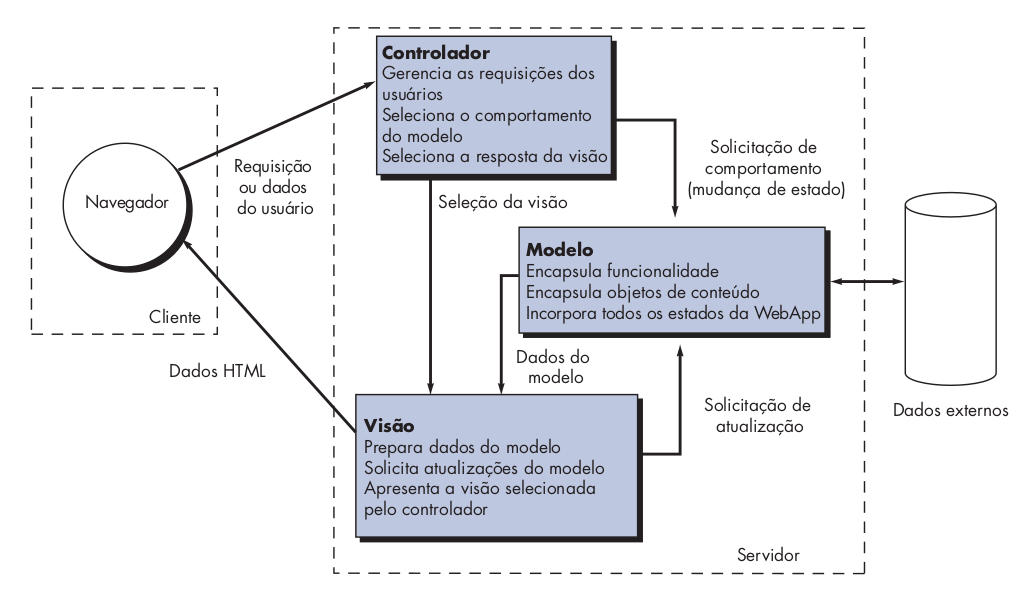
\includegraphics[scale=.45]{figuras/fig-ref-mvc} 
	\caption{Arquitetura MVC através de uma representação esquemática~\cite{pressman:es11}.}
	\label{fig-ref-mvc}
\end{figure}

O \textbf{(modelo)} apenas tem conhecimento sobre a lógica e os dados que estão armazenados no sistema através de bancos de dados ou arquivos. Ele é considerado o núcleo da aplicação e é onde as operações de CRUD podem ser realizadas. A \textbf{(visão)} não possui lógica de negócio e fica responsável por controlar a entrada dos dados fornecidos pelo usuário, devolvendo a saída das informações assim que elas forem repassadas pelo \textbf{(controlador)}. O \textbf{(controlador)} funciona como um intermediário, organizando os eventos enviados pela interface do usuário e os direcionando para o \textbf{(modelo)}.

O padrão MVC aborda dois tipos de separação. No primeiro tipo, existe uma separação entre a apresentação \textbf{(visão)} e a lógica de negócio \textbf{(modelo)}. No segundo tipo, o \textbf{(controlador)} é separado da \textbf{(visão)}, sendo este segundo tipo menos importante do que o primeiro. Como inúmeros sistemas possuem um único controlador por visão, o segundo tipo quase não é utilizado. Entretanto, o segundo tipo é mais comum em interfaces \textit{Web}, pois a parte de \textbf{(visão)} \textit{front end} é naturalmente separada do \textbf{(controlador)}~\cite{fowler:peaa02}.

De acordo com \citeonline{souza:masterthesis07}, a arquitetura MVC necessita de algumas alterações para atender as necessidades dos aplicativos \textit{Web}. O \textbf{(modelo)}, situado no servidor \textit{Web}, não consegue enviar as notificações das alterações para a \textbf{(visão)}, já que se encontra no navegador do lado do cliente e a comunicação é sempre iniciada pelo cliente. Então, apesar de MVC ser um nome bem conceituado, o nome correto para esse padrão arquitetônico, quando aplicado à \textit{Web}, seria ``Controlador Frontal'' (\textit{Front Controller})~\cite{alur-et-al:bpds03}. O padrão Controlador Frontal pode ser visualizado na Figura~\ref{fig-ref-controlador-frontal}.   

\begin{figure}[h]
	\centering
	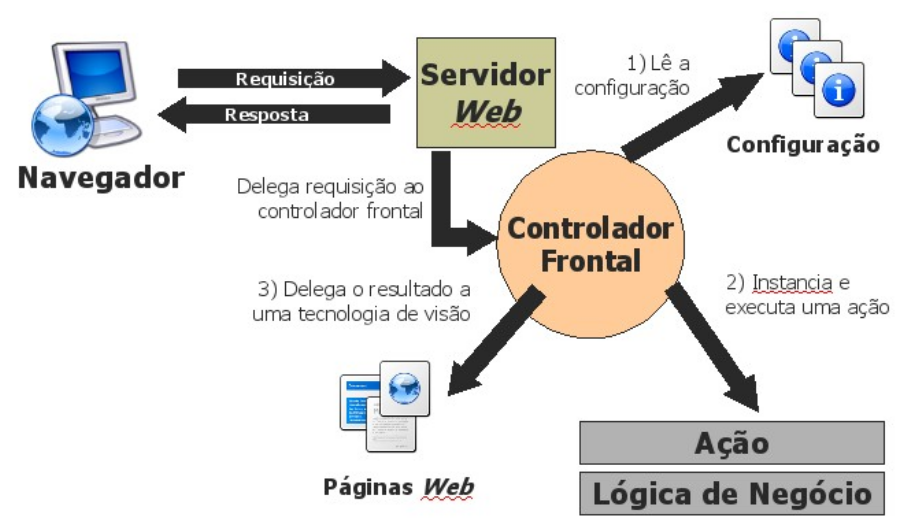
\includegraphics[scale=.45]{figuras/fig-ref-controlador-frontal} 
	\caption{Funcionamento do padrão arquitetônico Controlador Frontal na \textit{Web}~\cite{souza:masterthesis07}.}
	\label{fig-ref-controlador-frontal}
\end{figure}

\subsection{Framework Grails}
\label{sec-ref-framework-grails}

O Grails é um \textit{framework} voltado para o desenvolvimento de aplicações \textit{web}, baseado em MVC e que utiliza a linguagem Groovy. Com o objetivo de facilitar a vida dos desenvolvedores, a partir da utilização do Grails, a implementação da lógica de negócio passou a ser realizada de maneira imediata e sem a preocupação com a integração de inúmeras bibliotecas, como o Hibernate para a persistência, Spring e várias outras.

Visualizar de maneira instantânea o resultado das alterações em tempo de execução, também é uma característica do Grails. Algumas outras particularidades também podem ser mencionadas: as camadas de visualização e controle baseadas nas classes de domínio podem ser geradas automaticamente, a inversão de controle e a injeção de dependências são baseadas em Spring, os principais \textit{frameworks} e bibliotecas Java podem ser integrados facilmente e o \textit{framework} para persistência GORM fica responsável por controlar a validação dos dados, tirando a preocupação dos desenvolvedores com arquivos de mapeamento ou com anotações.

Após o projeto utilizando o \textit{framework} Grails ser finalizado, é possível obter como resultado uma aplicação Java EE completa, possuindo escalabilidade, robustez, desempenho e alta disponibilidade. Além disso, Grails é altamente portável entre servidores de aplicação~\cite{weissmann:fgapdw15}.       


\subsection{Linguagem Groovy}
\label{sec-ref-linguagem-groovy}


Alterar o comportamento do código enquanto ele é executado pode ser bem simples utilizando Groovy. Por se tratar de uma linguagem dinâmica e orientada a objetos, ela tem como vantagem a execução de tarefas em tempo de execução, se destacando com relação as outras linguagens que só executam através de padrões de projetos ou no momento da compilação. A linguagem Groovy é altamente compatível com os códigos desenvolvidos através da linguagem Java, que podem ser acessados transparentemente pelos códigos implementados em Groovy e vice-versa.

Com relação às variáveis que são utilizadas na linguagem, a definição dos tipos pode acontecer de modo estático ou dinamicamente, ou seja, a definição dos tipos das variáveis utilizadas no Groovy não é obrigatório. Os métodos são bem mais simples de serem definidos, pois não é preciso explicitar o tipo de retorno e nem utilizar a instrução return para retornar um valor.

No decorrer do Capítulo~\ref{sec-projeto} serão abordados mais alguns detalhes referentes a linguagem Groovy, que serão exemplificados de acordo como a demonstração da implementação do projeto.         



       